% ============================================================
% 5. EXPERIMENTS
% ============================================================
\vspace{-0.2in}
\section{Experiments}
\label{sec:experiments}

\subsection{Experimental Setup}
\label{sec:exp-setup}

We evaluate DIAL along three axes: does environment-aware gating improve the success-cost
frontier over fixed-direction baselines
(\S\ref{sec:main-results}); which components drive the gains
(\S\ref{sec:ablation}); and do the Two-Source Model's predictions
hold on held-out data (\S\ref{sec:theory-verification}).

\textbf{Environments.} We conduct evaluations across six environments: 
HotpotQA~\cite{yang2018hotpotqa},
APPS~\cite{hendrycks2021apps},
WebShop~\cite{yao2022webshop},
FEVER~\cite{thorne2018fever},
TWExpress~\cite{jansen2023twexpress}, and
Plancraft~\cite{dagan2024plancraft}. 
% , spanning QA, code generation,
% web navigation, fact verification, text games, and crafting planning.
These cover the full range of the Two-Source
Model, from intervention-unsuitable-leaning (FEVER) through mixed (WebShop) to decision-difficulty-leaning (APPS) settings, including extreme rollout properties
(TWExpress: rollout-safe; Plancraft: rollout-harmful).
Full environment specifications are in
Appendix~\ref{app:environment}.

\textbf{Baselines.} All methods share the same agent and
optimizer $T$; only the gating decision differs.
Six fixed-direction or fixed-budget baselines instantiate a
predetermined compute-allocation rule (high uncertainty, low
confidence, disagreement, or a fixed token budget triggering
additional computation):
CaTS~\cite{cats2025}, SEAG~\cite{seag2025},
CoRefine~\cite{corefine2026}, CATTS~\cite{catts2026},
AUQ~\cite{auq2026}, and s1\_budget~\cite{s1_2025}. Full specifications are in Appendix~\ref{app:method-comparison}. We additionally include two bounds for reference (Appendix~\ref{app:bounds-comparison}): \emph{base\_only}, which never triggers
the optimizer, and \emph{always\_trigger}.


\begin{table*}[h!]
\centering
\caption{Full results across 6 environments and 3 backbones. SR (\%) and Cost ($\times$base, total deployment tokens normalized by base\_only).
\textbf{Bold}: best SR per environment (excluding oracle).
$\dagger$: methods requiring calibration data.
Cost includes all LLM calls: base proposer, gate overhead (CATTS $K{=}5$ voting, AUQ confidence query), and rollout calls.
FEVER token costs are estimated.}
\label{tab:full-results}
\resizebox{\textwidth}{!}{%
\begin{tabular}{l *{6}{rc} }
\toprule
& \multicolumn{2}{c}{\textbf{HotpotQA}} & \multicolumn{2}{c}{\textbf{WebShop}} & \multicolumn{2}{c}{\textbf{FEVER}}
& \multicolumn{2}{c}{\textbf{TWExpress}} & \multicolumn{2}{c}{\textbf{Plancraft}} & \multicolumn{2}{c}{\textbf{APPS}} \\
\cmidrule(lr){2-3}\cmidrule(lr){4-5}\cmidrule(lr){6-7}
\cmidrule(lr){8-9}\cmidrule(lr){10-11}\cmidrule(lr){12-13}
\textbf{Method} & SR & $\times$b & SR & $\times$b & SR & $\times$b & SR & $\times$b & SR & $\times$b & SR & $\times$b \\
\midrule
\multicolumn{13}{c}{\textit{Qwen3-4B-Instruct}} \\
\midrule
base\_only        & 49.0 & 1.00 &  7.2 & 1.00 & 37.0 & 1.00 & 67.5 & 1.00 & 29.8 & 1.00 & 60.5 & 1.00 \\
always\_trigger   & 97.0 & 10.63 & 43.0 & 5.56 & 99.8 & 7.87 & 99.3 & 2.15 & 22.8 & 6.13 & 79.5 & 3.65 \\
CaTS$^\dagger$    & 93.2 & 10.54 & 30.5 & 3.45 & 50.2 & 25.48 & 96.7 & 1.37 & 22.3 & 4.14 & 66.2 & 1.61 \\
SEAG$^\dagger$    & 67.5 & 5.34 & 28.0 & 2.84 & 49.3 & 17.19 & 97.3 & 1.60 & 24.8 & 2.52 & 66.0 & 1.75 \\
CoRefine$^\dagger$& 68.2 & 5.28 & 27.5 & 2.78 & 49.8 & 17.19 & 97.5 & 1.57 & 22.8 & 2.44 & 67.5 & 1.70 \\
CATTS             & 68.3 & 10.53 & 16.0 & 5.55 & 34.2 & 6.46 & 97.5 & 2.83 & 25.0 & 6.53 & 60.8 & 6.00 \\
AUQ               & 97.0 & 10.29 & 35.7 & 5.83 & 40.7 & 8.04 & 95.5 & 1.35 & 24.2 & 6.64 & 64.7 & 3.28 \\
s1\_budget        & 97.0 & 6.27 &  7.8 & 1.91 & 46.2 & 9.21 & 95.0 & 0.93 & 18.3 & 2.02 & 69.0 & 2.15 \\
BSW               & 58.2 & 17.35 & 20.6 & 5.77 & 63.0 & 23.37 & 99.0 & 2.04 & 25.5 & 5.33 & 79.5 & 2.66 \\
\textbf{EAAG}     & \textbf{95.2} & 8.02 & \textbf{43.8} & 2.50 & 49.8 & 16.51 & \textbf{99.0} & 1.81 & 23.3 & 3.63 & \textbf{73.0} & 2.61 \\
\midrule
\multicolumn{13}{c}{\textit{Phi-3.5-mini-instruct}} \\
\midrule
base\_only        & 28.3 & --- &  3.5 & --- &  7.2 & --- & 66.7 & --- & 13.7 & --- & 27.0 & --- \\
always\_trigger   & 98.8 & --- & 53.5 & --- & 61.0 & --- & 97.8 & --- & 14.5 & --- & 79.5 & --- \\
CaTS$^\dagger$    & 68.3 & --- & 41.7 & --- & 19.8 & --- & 68.2 & --- & 13.5 & --- & 30.5 & --- \\
SEAG$^\dagger$    & 88.3 & --- & 36.5 & --- & 13.5 & --- & 94.5 & --- & 14.7 & --- & 27.8 & --- \\
CoRefine$^\dagger$& 87.7 & --- & 35.8 & --- & 13.7 & --- & 94.7 & --- & 15.2 & --- & 28.5 & --- \\
CATTS             & 42.0 & --- & 28.7 & --- & 12.7 & --- & 86.7 & --- & 13.5 & --- & 27.7 & --- \\
AUQ               & 31.2 & --- &  7.0 & --- &  8.5 & --- & 94.5 & --- & 12.7 & --- & 27.2 & --- \\
s1\_budget        & 94.2 & --- &  3.0 & --- & 23.0 & --- & 95.7 & --- & 13.7 & --- & 34.5 & --- \\
\textbf{EAAG}     & \textbf{92.3} & --- & \textbf{57.3} & --- & 16.5 & --- & \textbf{96.7} & --- & 13.8 & --- & \textbf{36.8} & --- \\
\midrule
\multicolumn{13}{c}{\textit{Llama-3.1-8B-Instruct}} \\
\midrule
base\_only        & 46.3 & --- &  1.2 & --- & 13.2 & --- & 36.5 & --- & 31.7 & --- & 60.2 & --- \\
always\_trigger   & 99.5 & --- & 42.8 & --- & 62.8 & --- & ---  & --- & 18.7 & --- & 79.5 & --- \\
CaTS$^\dagger$    & 96.2 & --- & 36.0 & --- & 56.3 & --- & ---  & --- & 22.8 & --- & 60.2 & --- \\
SEAG$^\dagger$    & 96.0 & --- & 27.5 & --- & 53.3 & --- & 76.5 & --- & 21.8 & --- & 60.2 & --- \\
CoRefine$^\dagger$& 96.2 & --- & 27.5 & --- & 53.5 & --- & 76.0 & --- & 21.5 & --- & 60.2 & --- \\
CATTS             & 96.0 & --- &  1.3 & --- & 14.2 & --- & 49.3 & --- & 27.0 & --- & 52.3 & --- \\
AUQ               & 97.0 & --- & 37.8 & --- & 52.8 & --- & 63.2 & --- & 27.0 & --- & 60.0 & --- \\
s1\_budget        & 96.5 & --- &  1.2 & --- & 13.8 & --- & ---  & --- & 30.3 & --- & 72.5 & --- \\
\textbf{EAAG}     & \textbf{95.5} & --- & \textbf{41.7} & --- & 34.7 & --- & \textbf{94.8} & --- & 27.0 & --- & 59.7 & --- \\
\bottomrule
\end{tabular}%
}
\end{table*}


\textbf{Metrics.} We use SR (success rate, $\uparrow$) and Cost
($\times$base, $\downarrow$): total deployment tokens normalized by
base\_only tokens per episode. This metric counts \emph{all} LLM
calls, including base proposer, gate overhead, and rollout calls, ensuring that per-step
overhead is not hidden. Calibration or exploration overhead is
excluded for all methods.
A method Pareto-dominates another if $\text{SR} \geq$ and
$\text{Cost} \leq$ with at least one strict inequality.
Token cost constants are reported in
Appendix~\ref{app:cost}.
\vspace{-0.1in}
\subsection{Main Results}
\label{sec:main-results}
\vspace{-0.1in}


\textbf{DIAL improves the success-cost frontier over fixed-direction baselines.}
Table~\ref{tab:full-results} reports SR and Cost ($\times$base) across all 6 environments and 3 backbones; the Qwen3-4B Pareto frontier is visualized in Appendix~\ref{app:multi-backbone}. DIAL
achieves the highest SR in 16 of 18 (environment, backbone) cells. Three insights follow.
First, \emph{wrong direction is catastrophic, not merely costly}.
On Qwen3-4B FEVER, an intervention-unsuitable-leaning environment, CATTS pays 16.46$\times$ base for $K{=}5$ voting yet reaches only 32.2\% SR, below the 37.0\% no-trigger baseline: fixed-direction gating in the wrong direction
does not merely waste compute, it actively hurts.
Second, \emph{learning the right direction yields a better SR-cost trade-off, not just a retuned threshold}. On Qwen3-4B HotpotQA, DIAL trades 1.8 SR points for 2.6$\times$ less cost than always\_trigger (95.2 vs.\ 97.0\% at 8.02$\times$ vs.\ 10.63$\times$); on WebShop, DIAL matches always\_trigger at less than half the cost. The gap is too large
to close by retuning thresholds without changing direction.
Third, \emph{the win generalizes across backbones}. The same DIAL pipeline takes 6/6 cells on both Qwen3-4B and Phi-3.5-mini and 4/6 on Llama-3.1-8B, even though entropy--utility correlations flip sign across model families (\S\ref{sec:empirical-landscape}). Fixed-direction baselines instead break per-backbone: AUQ on HotpotQA falls from 95.0\% (Qwen3-4B) to 31.2\% (Phi-3.5).



% FEVER remains DIAL's weakest environment: while DIAL achieves the
% highest SR (49.8\%), its cost (16.51$\times$base) is also the
% highest, a limitation we analyze in \S\ref{sec:discussion}.
\vspace{-0.1in}
\subsection{Ablation Studies}
\label{sec:ablation}
\vspace{-0.1in}
The main results show that DIAL works; we now ask
\emph{why}. We ablate direction along two axes: its sign
(direction reversal) and the gate's capacity to exploit it
(gate complexity). We then characterize how DIAL's trigger
rate adapts across rollout-headroom regimes and explain why fewer
rollouts can improve accuracy. LLM feature and
regularizer ablations appear in Appendix~\ref{app:llm-features}
and Appendix~\ref{app:regularizer-ablation}.

\begin{wraptable}{r}{0.52\textwidth}
\vspace{-1pt}
\caption{Effect of reversing DIAL's learned direction.
$\Delta$SR: reversed $-$ original. $|\rho_{\text{ent}}|$ is the
absolute Spearman correlation between token entropy and
optimizer utility. Degradation scales with $|\rho_{\text{ent}}|$.}
\vspace{-.1in}
\label{tab:wrong-direction}
\centering
\resizebox{0.5\textwidth}{!}{%
\begin{tabular}{lcccc}
\toprule
Environment & DIAL SR & Reversed SR & $\Delta$ SR & $|\rho_{\text{ent}}|$ \\
\midrule
FEVER          & 49.8\% & 13.0\% & $-$36.8 & 0.619 \\
HotpotQA       & 95.2\% & 58.2\% & $-$37.0 & 0.494 \\
WebShop        & 43.8\% & 20.6\% & $-$23.2 & 0.444 \\
APPS           & 73.0\% & 70.5\% & $-$2.5  & 0.339 \\
TWExpress      & 99.0\% & 96.2\% & $-$2.8  & 0.290 \\
Plancraft      & 23.3\% & 20.5\% & $-$2.8  & 0.016 \\
\bottomrule
\end{tabular}%
}
\vspace{-10pt}
\end{wraptable}
\textbf{Direction is a first-order determinant of gate quality.}
To isolate the effect of direction, we reverse the sign of all learned weights in DIAL's fitted gate while keeping everything
else unchanged, constructing an adversarially wrong-direction gate that preserves ranking structure but inverts trigger
semantics. Table~\ref{tab:wrong-direction} shows that on strong-signal environments with $|\rho_{\text{ent}}| > 0.4$,
reversal collapses SR by 23--37\%; on weak-signal Plancraft ($|\rho_{\text{ent}}|{=}0.016$) the effect is negligible. The damage scales with signal strength: wrong direction is not a calibration error but a structural failure. This instantiates the
wrong-direction harm result of Appendix~\ref{app:wrong-direction}: a sharper gate fires precisely on the states where
computation has negative value.

\begin{wrapfigure}{r}{0.45\textwidth}
\vspace{-12pt}
\centering
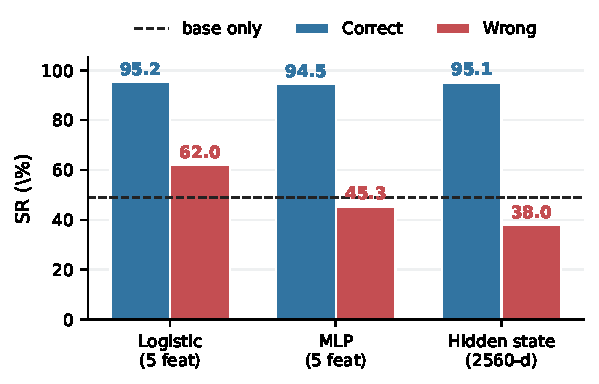
\includegraphics[width=0.43\textwidth]{figures/fig_capacity_ablation.pdf}
\vspace{-0.1in}
\caption{Gate complexity ablation on HotpotQA (Qwen3-4B). With
correct direction all gates reach $\approx$95\%; with
wrong direction.}
\label{fig:capacity}
\vspace{-10pt}
\end{wrapfigure}
\textbf{Gate capacity does not substitute for direction.}
A natural objection is that DIAL's gains come from gate simplicity rather than learned direction. With correct
direction, a logistic gate, a 2-layer MLP, and a hidden-state probe (2560-d) all reach $\approx$95\% SR on HotpotQA: capacity adds $<$1\% (Figure~\ref{fig:capacity}). With wrong direction, the ordering inverts: the MLP drops to 45.3\%, \emph{below} the wrong-direction logistic at 62.0\%. Direction consistently outweighs capacity, which is why DIAL's minimal linear gate suffices.

\textbf{Trigger rate adapts to rollout headroom.}
In rollout-harmful environments, baselines that fire aggressively pay a price beyond efficiency: on Plancraft
($\Delta{=}{-}7.0$), s1\_budget keeps triggering and falls below \emph{base\_only} (16.3\% vs.\ 29.8\%, see
Appendix~\ref{app:bounds-comparison}); more compute makes performance \emph{worse} than no gate at all. DIAL avoids this trap without ever observing the headroom: its trigger rate adapts from 73\% on rollout-safe TWExpress, where almost any
trigger helps, down to $<$20\% on Plancraft, with a within-episode decay from 49\% at step~0 to under 20\% in late
steps as the gate learns that further rollouts only add harm. This adaptive magnitude emerges from the per-environment signed weights alone: direction discovery already encodes whether the environment rewards or penalizes additional computation. The full per-step analysis is in Appendix~\ref{app:trigger-rate}.

\textbf{Why fewer rollouts can improve SR.}
The optimizer is not a monotone improvement operator. In intervention-unsuitable states, rollout evaluation starts from the same unreliable context as the base policy and can amplify misleading evidence, invalid intermediate states, or compounding trajectory errors. Avoiding such negative-utility interventions therefore improves accuracy, not merely efficiency. DIAL's gain in low-headroom regimes comes from learning when \emph{not} to invoke the optimizer, while still triggering in decision-difficult states where rollouts expose useful alternatives.


\vspace{-0.1in}
\subsection{Two-Source Model Verification}
\vspace{-0.1in}
\label{sec:theory-verification}
\begin{wrapfigure}{r}{0.5\textwidth}
	\vspace{-12pt}
	\centering
	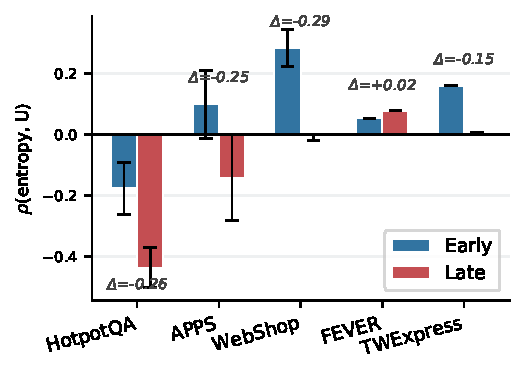
\includegraphics[width=0.43\textwidth]{figures/fig_temporal_shift.pdf}
	\vspace{-0.1in}
	\caption{P1: $\rho$(entropy, $U$) shifts from early (blue,
		step $\leq$ median) to late (red); bars show Spearman $\rho$.
		Plancraft omitted ($|\rho|{=}0.016$).}
	\label{fig:temporal-shift}
	\vspace{-10pt}
\end{wrapfigure}
The empirical landscape (\S\ref{sec:empirical-landscape}) shows
direction varies but does not pin down the Two-Source Model
(\S\ref{sec:toy-model}) as the cause. We test the model with
three complementary experiments that each rule out a different
class of alternative explanation: within-episode temporal
dynamics (P1, observational), within-task causal manipulation
of the information mixture (P2, interventional), and
cross-environment alignment of the dominant signal with the
dominant state type (P3, population-level).


\textbf{P1: Temporal dynamics.}
The Two-Source Model predicts that $\rho$ should decrease over the episode: as the agent gathers information, Type~D states are resolved and late-step uncertainty increasingly reflects residual Type~I states.
Figure~\ref{fig:temporal-shift} supports this pattern in environments with strong temporal signal. In HotpotQA, $\rho$ shifts from $-0.176$ (early) to $-0.437$ (late). In
WebShop, the strong positive early-phase signal ($\rho{=}{+}0.285$) vanishes in the late phase. In APPS, $\rho$ shifts from non-significant positive ($+$0.102) to weak negative ($-$0.144). Full results are in
Appendix~\ref{app:temporal}.

%\vspace{-0.05in}
\begin{wraptable}{r}{0.5\textwidth}
\vspace{-12pt}
\caption{Controlled information manipulation on HotpotQA
(Qwen3-4B): availability shifts which signal dominates,
providing causal evidence for the Two-Source Model.}
\vspace{-0.05in}
\label{tab:controlled}
\centering\footnotesize
\setlength{\tabcolsep}{4pt}
\begin{tabular}{lcccc}
\toprule
Condition & Base SR & $\rho$(ent.) & $\rho$(step) & DIAL SR \\
\midrule
Original  & 49.0\% & $-$0.041 & $-$0.494 & 95.2\% \\
InfoPoor  & 44.0\% & $+$0.119 & $\mathbf{-0.608}$ & 94.0\% \\
InfoRich  & 82.0\% & $\mathbf{+0.311}$ & $-$0.147 & 88.3\% \\
\bottomrule
\end{tabular}
\vspace{-10pt}
\end{wraptable}
\textbf{P2: Controlled information manipulation.} P1 verifies a within-episode dynamic; we now intervene on $p_I$ directly for \emph{causal} evidence. We construct two
interventions on HotpotQA: \textbf{InfoPoor} restricts retrievable evidence to a small passage subset (increasing the Type~I mixture), and \textbf{InfoRich} prepends gold-standard evidence to the prompt (reducing one major source of intervention-unsuitability, namely information poverty, and shifting states toward Type~D). Table~\ref{tab:controlled}
reports the result: restricting evidence makes \texttt{step\_count} dominant ($\rho{=}{-}0.608$) while entropy
is weak; injecting gold evidence makes entropy dominant ($\rho{=}{+}0.311$) while \texttt{step\_count} weakens. As the
only test in this section that intervenes on the latent mixture rather than observing it, P2 confirms that signal identity is a function of information structure.
%, not an
%environment-specific constant.
%\vspace{-0.05in}

\begin{wraptable}{r}{0.6\textwidth}
\vspace{-12pt}
\caption{Strongest signal per environment aligns with the
dominant regime: information-sufficiency proxies in Type~I,
decision-complexity in Type~D.}
\vspace{-0.05in}
\label{tab:signal-identity}
\centering\footnotesize
\setlength{\tabcolsep}{3pt}
\begin{tabular}{lllcl}
\toprule
\textbf{Env} & \textbf{Regime} & \textbf{Strongest Signal} & $|\rho|$ & \textbf{Interpretation} \\
\midrule
HotpotQA   & Type~I & step\_count        & 0.494 & Info accumulation \\
FEVER      & Type~I & step\_count        & 0.619 & Info accumulation \\
TWExpress  & Type~I & step\_count        & 0.477 & Exploration depth \\
WebShop    & Mixed  & num\_avail\_actions & 0.444 & Decision-space size \\
APPS       & Type~D & step\_count        & 0.339 & Debugging depth \\
Plancraft  & Weak   & has\_output        & 0.162 & Rollout harmful \\
\bottomrule
\end{tabular}
\vspace{-10pt}
\end{wraptable}
\textbf{P3: Signal identity alignment.}
P2 manipulated information within one task; P3 asks whether the
predicted alignment also holds \emph{across} tasks. The
Two-Source Model further predicts that the strongest signal in
each environment should reflect its dominant state type:
information-sufficiency proxies in Type~I, decision-complexity
proxies in Type~D. Table~\ref{tab:signal-identity} confirms this: \texttt{step\_count} dominates in Type~I environments,
while \texttt{num\_available\_actions} and other choice-related features dominate in WebShop. The LASSO coefficient matrix and its interpretation as Two-Source proxies are in Appendix~\ref{app:feature-selection}.

The three tests are observational, interventional, and
population-level respectively, and rule out distinct confounds.
Cross-setting $\rho$ consistency at fixed backbone is reported
in Appendix~\ref{app:cross-setting}, and multi-backbone
verification in Appendix~\ref{app:multi-backbone} provides
additional robustness checks.

% Tables tab:controlled and tab:signal-identity moved inline as wraptables in P2 and P3.


